%%
%% Copyright (c) 2018 The Authors.  All Rights Reserved.
%%
%% Weitian LI, et al.
%% School of Physics and Astronomy, Shanghai Jiao Tong University,
%% Shanghai, China.
%%
%% 2018-08-23
%%

\documentclass[letters,a4paper,fleqn,usenatbib]{mnras}
% Available options:
% - letters : for papers in the journal's Letters section (<=5 pages)
% - onecolumn : single column
% - doublespacing : double line spacing (do NOT submit in this format)
% - usenatbib : (always use this) use `natbib' package for citations
% - usegraphicx : includes the `graphicx' package
% - useAMS : support 3 upright Greek characters
% - usedcolumn : use `dcolumn' package for table column alignment

% Chinese
\usepackage{xeCJK}
\setCJKmainfont{Noto Serif CJK SC}[BoldFont=Noto Sans CJK SC]
\setCJKsansfont{Noto Sans CJK SC}

\usepackage{newtxtext,newtxmath}
\usepackage[T1]{fontenc}
\usepackage{ae,aecompl}

%
% Custom packages
%
\usepackage{graphicx}
\usepackage{amsmath}
\usepackage{amssymb}
\usepackage{siunitx}  % typeset units; from `texlive-science'

\graphicspath{{./}{figures/}}  % NOTE: the trailing '/' matters

\sisetup{
  range-phrase=\text{--},
  range-units=single,
  product-units=repeat,
  list-separator={, },
  list-final-separator={, and },
  separate-uncertainty=true,
}
\DeclareSIUnit\MHz{\mega\hertz}
\DeclareSIUnit\kHz{\kilo\hertz}
\DeclareSIUnit\jansky{Jy}
\DeclareSIUnit\mJy{\milli\jansky}

\def\sectionautorefname{Section}
\def\subsectionautorefname{Section}
\def\figureautorefname{Fig.}
\def\tableautorefname{Table}

%
% Custom commands
%
\newcommand{\R}[1]{\mathrm{#1}}
\newcommand{\B}[1]{\mathbfit{#1}}
\newcommand{\M}[1]{\mathbfss{#1}}


%%======================================================================
%% Title page
%%

%      ............................................. (<=45 chars)
\title[EoR Separation with CDAE]{%
  Deep-learning-based Method to Separate the EoR Signal
  Using the Convolutional Denoising Autoencoder
}

% If you need two or more lines of authors, add an extra line using \newauthor
\author[Li~et~al.]{%
Weitian Li,$^{1}$\thanks{E-mail:
  \href{mailto:liweitianux@sjtu.edu.cn}{liweitianux@sjtu.edu.cn} (WL);
  \href{mailto:hgxu@sjtu.edu.cn}{hgxu@sjtu.edu.cn} (HX)}
Haiguang Xu,$^{1,2,3}$\footnotemark[1]
Zhixian Ma,$^{4}$
Ruimin Zhu,$^{5}$
Dan Hu,$^{1}$
Zhenghao Zhu,$^{1}$
\newauthor
Chenxi Shan,$^{1}$
Jie Zhu$^{4}$
and
Xiang-Ping Wu$^{6}$
\\
% List of institutions
$^{1}${School of Physics and Astronomy,
  Shanghai Jiao Tong University,
  800 Dongchuan Road, Shanghai 200240, China} \\
$^{2}${Tsung-Dao Lee Institute,
  Shanghai Jiao Tong University,
  800 Dongchuan Road, Shanghai 200240, China} \\
$^{3}${IFSA Collaborative Innovation Center,
  Shanghai Jiao Tong University,
  800 Dongchuan Road, Shanghai 200240, China} \\
$^{4}${Department of Electronic Engineering,
  Shanghai Jiao Tong University,
  800 Dongchuan Road, Shanghai 200240, China} \\
$^{5}${Department of Statistics,
  Northwestern University,
  2006 Sheridan Road, Evanston, IL 60208, US} \\
$^{6}${National Astronomical Observatories,
  Chinese Academy of Sciences,
  20A Datun Road, Beijing 100012, China}
}

% These dates will be filled out by the publisher
\date{Accepted XXX. Received YYY; in original form ZZZ}

% Enter the current year, for the copyright statements etc.
\pubyear{2018}

% Don't change these lines
\begin{document}
\label{firstpage}
\pagerange{\pageref{firstpage}--\pageref{lastpage}}
\maketitle

%
% Abstract
% (<=200 words for Letters)
%
\begin{abstract}
The overwhelming foreground contamination is one of the primary
challenge in measuring the \SI{21}{\cm} signal to probe the EoR.
Although the foreground is expected to be spectrally smooth,
the frequency-dependent beam effects of interferometers can
seriously damage the smoothness of foreground spectrum,
imposing great difficulties on existing foreground removal methods.
In this work, we propose a novel deep-learning-based method by employing
the convolutional denoising autoencoder (CDAE) to separate the EoR signal.
The proposed CDAE, which consists of a 7-layer encoder, a 7-layer
decoder, and one output layer, is simple but powerful and successfully
learns robust features of the faint EoR signal that is contaminated by the
severe foreground emission.
By training and evaluating the CDAE on the simulated SKA images, it
achieves excellent performance with the correlation coefficient between
the separated EoR signal and the simulated `true' signal being
$\rho_{\R{cdae}} = \num{0.985 +- 0.009}$.
As a comparison, the traditional polynomial fitting method has very poor
performance ($\rho_{\R{pfit}} = \num{0.241 +- 0.103}$ on the same data set).
In conclusion, our deep-learning-based method can accurately separate
the faint EoR signal in the presence of severe foreground contamination
and complicated instrumental effects.
\end{abstract}

% Select between one and six entries from the list of approved keywords.
% Don't make up new ones.
% https://academic.oup.com/DocumentLibrary/mnras/keywords.pdf
\begin{keywords}
methods: data analysis --
techniques: interferometric --
dark ages, reionization, first stars --
radio continuum: general
\end{keywords}


%%======================================================================
%% Paper body
%%

\section{Introduction}
\label{sec:intro}

The \SI{21}{\cm} line emission of the neutral hydrogen,
which is believed to be redshifted to frequencies below \SI{200}{\MHz},
is regarded as a decisive probe to directly explore the epoch of
reionization (EoR), a period of the early Universe
($z \sim \numrange{6}{15}$) that is still poorly understood
\citep[see][for reviews]{furlanetto2006rev,furlanetto2016rev}.
As of today, several low-frequency radio interferometers have been built
or under construction to target the \SI{21}{\cm} signal, including
21CMA \citep{zheng2016}, GMRT \citep{paciga2011}, MWA \citep{tingay2013},
LOFAR \citep{vanHaarlem2013}, PAPER \citep{parsons2010},
HERA \citep{deboer2017}, and SKA \citep{koopmans2015rev}.
The observational challenges, however, are immense due to a variety of
complicated instrumental effects, ionospheric distortions, radio frequency
interference, and the strong astronomical foreground contamination that
overwhelms the EoR signal by about \numrange{4}{5} orders of magnitude
\citep[see][for a review]{morales2010rev}.

Fortunately, in the frequency dimension, the foreground contamination
is expected to be very smooth, while the EoR signal fluctuates rapidly
on scales of $\lesssim \si{\MHz}$.
This important difference is the key characteristic exploited by many
foreground removal methods in order to uncover the faint EoR signal,
including
parametric fitting methods \citep[e.g.,][]{wang2006,liu2009fgrm,wang2013}
and non-parametric methods \citep[e.g.,][]{harker2009,chapman2013,mertens2018}.

However, the frequency-dependent beam effects can damage the smoothness
of the foreground spectra \citep{liu2009ps}.
The point spread function (PSF), which is the Fourier Transform (FT)
of the interferometer layout, varies with observing frequencies and
has jagged side-lobes extending far beyond the main lobe due to the
incomplete $uv$ coverage.
Therefore, an unresolved or mis-subtracted source can leave residuals
at different positions in the cleaned images of different frequencies.
As a result, every pixel in the obtained image cube has unpredictable
oscillating residuals along the frequency dimension, imposing great
difficulties on the foreground removal methods that rely on the
smoothness of the foreground contamination \citep[see also][]{liu2009ps}.

Given the complicated profiles and frequency-dependent variations of
the PSF, it is extremely difficult to craft a parametric model for
existing foreground removal methods to overcome the intricate beam
effects, thus the data-driven modelling method is more feasible and
appealing [这主要是我们自己的观点、未找到相关文献可引].
In recent years, the deep learning algorithms have seen prosperous
developments and brought breakthroughs into a variety of fields, such
as image classification, speech recognition, and object detection
\citep[see][for a recent review]{lecun2015}.
Among all kinds of neural network architectures, the autoencoder
is able to learn robust features in the data \citep{vincent2008}
and has been widely applied to
dimensionality reduction \citep{hinton2006},
image inpainting and denoising \citep{suganuma2018},
speech separation \citep{grais2017}, and so on.

In this paper, in order to tackle the intricate frequency-dependent
beam effects, we propose a novel deep-learning-based method to separate
the EoR signal along the frequency dimension by making use of the
convolutional denoising autoencoder (CDAE), a popular variant of
autoencoders that is designed to recover the original clean signal
from the noisy data.
To the best of our knowledge, there is no similar deep-learning-based
methods for the EoR signal separation in the literature.
In \autoref{sec:method}, we briefly introduce the CDAE and elaborate
the proposed method.
In \autoref{sec:experiments}, we demonstrate the performance of the
method by applying it to the simulated SKA images.
We discuss the method and carry out a comparison to the traditional
polynomial fitting method in \autoref{sec:discussions}.
Finally, we conclude our work in \autoref{sec:conclusions}.
The implementation code and data are made public at
\url{https://github.com/lwieitianux/cdae-eor}.


%%======================================================================
\section{Methodology}
\label{sec:method}

%%----------------------------------------------------------------------
\subsection{Convolutional denoising autoencoder}
\label{sec:cdae}

An autoencoder is composed of two parts: the encoder and the decoder,
which can be described by two functions $f(\cdot)$ and $g(\cdot)$,
respectively.
The encoder maps the input $\B{x}$ to an internal code $\B{h}$, i.e.,
$\B{h} = f(\B{x})$, while the decoder tries to reconstruct the input
from the code $\B{h}$, i.e., $\B{r} = g(\B{h})$.
By placing constraints (e.g., dimensionality, sparsity) on the
internal code $\B{h}$ and training the autoencoder to minimise the
loss $L(\B{x}, \B{r})$, which quantifies the difference between the
reconstruction $\B{r}$ and the input $\B{x}$, the autoencoder is able
to learn the codes that effectively represent the input data
\citep[chapter 14]{goodfellow2016}.

The CDAE combines the ideas of both the convolutional neural network
and the denoising autoencoder \citep{du2017}.
The use of multiple convolutional layers improves the ability of the
CDAE to extract sophisticated features in the data \citep{masci2011}.
Training the CDAE on the noisy data $\B{\~{x}}$ forces the CDAE to
learn features that are robust to the noise in the data, thus the
trained CDAE can recover the original data $\B{x}$ from the noisy
input $\B{\~{x}}$ \citep{vincent2008,vincent2010}.

In the task of separating the EoR signal, the foreground contamination,
albeit very strong, can be regarded as the noise that corrupts the
target signal.
Therefore, the CDAE is the appropriate deep-learning method to extract
the features of the faint EoR signal that are robust to the foreground
contamination and the frequency-dependent beam effects.


%%----------------------------------------------------------------------
\subsection{Network architecture}
\label{sec:architecture}

We propose a deep CDAE for separating the EoR signal, as shown
in \autoref{fig:network}.
The CDAE consists of a 7-layer encoder, a 7-layer decoder,
and one output layer.
The encoder and decoder parts are symmetric and use the rectified
linear unit (ReLU) as the activation function, while the output layer
uses the `tanh' activation function (see also \autoref{sec:data}).
All the convolutional layers have filters of size 3 and the filters
are one-dimensional (1D) because of the 1D input data, i.e., along the
observing frequency dimension.

\begin{figure}
  \centering
  \includegraphics[width=\columnwidth]{network-crop}
  \caption{\label{fig:network}%
    The network architecture of the proposed CDAE that
    predicts the clean EoR signal from the noisy signal corrupted by
    the foreground.
    The CDAE consists of a 7-layer encoder (the orange boxes),
    a 7-layer decoder (the blue boxes), and one output layer
    (the green box).
    All the convolutional layers use 1D filters of size 3, and
    the number of filters in each layer is shown in the boxes
    with bold font.}
\end{figure}


%%----------------------------------------------------------------------
\subsection{Data preprocessing}
\label{sec:data}

To better train the CDAE, the data should be appropriately preprocessed.
The raw input data are an image cube that covers a frequency band and
contains both the EoR signal and foreground contamination.
Each pixel of the image cube is represented by a vector, which is one
data point to be input to the CDAE.
Given the important difference in spectral structures between the EoR
signal and the foreground emission, we apply the Fourier Transform to
the raw data along the frequency dimension to make the EoR signal more
distinguishable and easier to learn by the CDAE.
The Blackman-Nuttall window function is applied to suppress the side-lobes
in the Fourier Transform caused by the sharp discontinuities at the ends
of the finite frequency band \citep[e.g.,][]{chapman2016}.
The $n_{\R{ex}}$ lowest Fourier components, which generally have large
values and are almost contributed by the spectral-smooth foreground
emission, are excised not only to avoid the higher Fourier components
where the EoR signal mainly resides being overwhelmed, but also to
make the pixels have similar weights to the CDAE.
To be able to reconstruct the separated EoR signal, both the real and
imaginary parts of the Fourier coefficients must be used in the CDAE,
therefore, the real and imaginary parts are separated and concatenated
into a new vector.
Finally, the data are zero-centred and normalised to have unit variance.

On the other hand, the preprocessing steps for the labelled data (i.e.,
the image cube of the EoR signal only) are similar to the above steps
but need minor adjustments.
After applying the Fourier Transform, excising the $n_{\R{ex}}$ lowest
components, and concatenating the real and imaginary parts,
the labelled data are truncated within the 1$^{\R{th}}$ and 99$^{\R{th}}$
percentiles to remove possible extreme values, and then divided by the
maximum absolute value of the truncated data.
In this way, the sign of the labelled data is preserved for the purpose
of reconstruction and the value range is constrained within $[-1, 1]$,
which allows us to use the `tanh' activation function for the output
layer in the CDAE.


%%----------------------------------------------------------------------
\subsection{Training}
\label{sec:training}

By training the CDAE to minimise the loss, which describes the
difference between the output of the CDAE and the labelled data,
the CDAE is able to predict the expected output from the input data.
The loss of the proposed CDAE is calculated as the
`mean squared error' (MSE).
The CDAE is initialised by the Glorot uniform initialiser \citep{glorot2010}
and is trained using the Adam optimisation method \citep{kingma2015}.


%%----------------------------------------------------------------------
\subsection{Evaluation index}
\label{sec:index}

To evaluate the performance of separating the EoR signal, the Pearson's
correlation coefficient is adopted to measure the similarity between
the separated signal $\mathbf{s}_p$ and the ground truth $\mathbf{s}_t$
(i.e., the labelled data):
\begin{equation}
  \label{eq:corrcoef}
  \rho(\mathbf{s}_p, \mathbf{s}_t) =
    \frac{\sum_{i=1}^{n}(s_{p,i}-\bar{s}_p)(s_{t,i}-\bar{s}_t)}{
      \sqrt{\sum_{i=1}^{n}(s_{p,i}-\bar{s}_p)^2
        \sum_{i=1}^{n}(s_{t,i}-\bar{s}_t)^2}
    },
\end{equation}
where $\bar{s}_p$ and $\bar{s}_t$ are the mean values.
The closer the correlation coefficient is to one, the better the
performance of separation.


%%======================================================================
\section{Experiments}
\label{sec:experiments}

%%----------------------------------------------------------------------
\subsection{Data simulation}
\label{sec:simulation}

In order to derive the data set to train the proposed CDAE and evaluate
its performance, we carry out end-to-end simulations to generate the
`observed' image cubes.
Following our previous works \citep{wang2010,wang2013}, we simulate the
\SIrange{154}{162}{\MHz} sky images of the foreground emission,
which includes the Galactic synchrotron and free-free emissions,
extragalactic point sources, and radio haloes.
The sky maps of the EoR signal are created using the 2016 data release
from the Evolution Of 21~cm Structure project \citep{mesinger2016}.
The sky images cover a sky patch of size \SI{10 x 10}{\degree} and have
a pixel size of \SI{20}{\arcsecond} (i.e., \num{1800 x 1800} pixels).
The \SIrange{154}{162}{\MHz} frequency band is divided into 101
channels with a frequency resolution of \SI{80}{\kHz} to better
preserve the spectral structures of the EoR signal.
Note that the bright point sources that have a flux density
$S_{158} > \SI{10}{\mJy}$ at \SI{158}{\MHz} are assumed to be
removed \citep[e.g.,][]{liu2009ps}.

To take into account the practical instrumental effects of radio
interferometers, the SKA1-Low layout configuration\footnote{%
  SKA1-Low Configuration Coordinates:
  \url{https://astronomers.skatelescope.org/wp-content/uploads/2016/09/SKA-TEL-SKO-0000422_02_SKA1_LowConfigurationCoordinates-1.pdf}
  (released on 2016 May 21)}
is employed to simulate the `observed' images.
Specifically, the \textsc{oskar}\footnote{%
  OSKAR: \url{https://github.com/OxfordSKA/OSKAR} (version 2.7.0)}
simulator \citep{mort2010} is used to perform the simulated
observations for \SI{6}{\hour}.
The visibility data are then imaged by the \textsc{wsclean}\footnote{%
  WSClean: \url{https://sourceforge.net/p/wsclean} (version 2.5)}
imager \citep{offringa2014} using the natural weighting and baseline
range of \numrange{30}{1000} wavelengths to emphasise the faint diffuse
EoR signal.
Only the central \SI{2 x 2}{\degree} regions (i.e., \num{360 x 360}
pixels) of the created images are cropped out for use in this work.

Therefore, we obtain two image cubes of dimension \num{360 x 360 x 101}
for the EoR signal and the foreground emission, respectively.
The spectra of two example pixels are shown in \autoref{fig:simudata},
where the absolute differences between two adjacent frequencies are
also plotted for the foreground emission.
It is clearly shown that the smoothness of the foreground spectrum is
seriously damaged by the instrumental effects.

The input data for the CDAE are the addition of the two image cubes,
i.e., both the EoR signal and the foreground contamination,
and the labelled data are the image cube of the EoR signal.
The total number of data points in this data set, i.e., the number of
pixels of the image cubes, is 129,600.

\begin{figure}
  \centering
  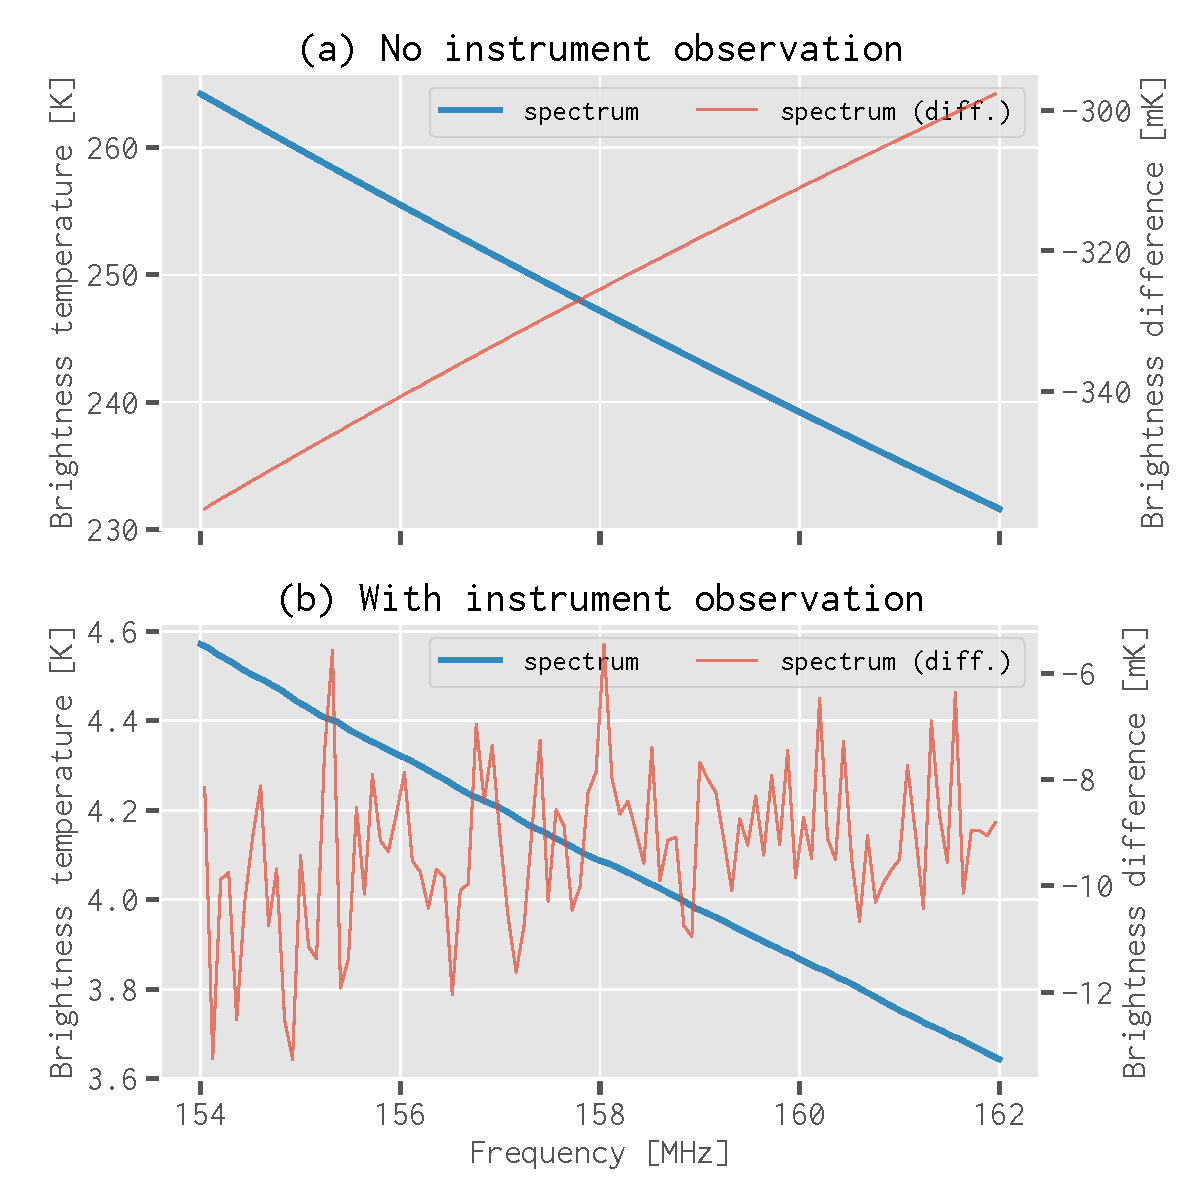
\includegraphics[width=\columnwidth]{simudata}
  \caption{\label{fig:simudata}%
    The spectra of two example pixels in the simulated image cubes
    for the EoR signal (the top panel) and the foreground emission
    (the bottom panel).
    The thin lines in the bottom panel show the absolute differences
    between two adjacent frequencies for the foreground emission.
  }
\end{figure}


%%----------------------------------------------------------------------
\subsection{Method implementation}
\label{sec:implementation}

We first preprocess the simulated data according to the steps described
in \autoref{sec:data}.
It is sufficient to keep only half the Fourier coefficients because the
input signal is real.
The data of length 101 for one pixel is transformed to be
51 complex Fourier coefficients, among which the $n_{\R{ex}} = 6$
coefficients of the lowest Fourier frequencies are excised.
Thus the length of each preprocessed data point is 90.
The data set is then randomly divided into two parts:
(1) the training set, which has 103,680 data points, accounting for
80 per cent of the whole data set;
(2) the validation set, containing the remaining 25,920 data points.

We implement the CDAE using the \textsc{Keras} framework \citep{keras}
with the \textsc{TensorFlow} back end \citep{tensorflow}.
The parameters of Adam optimisation method are set to the recommended
default values, i.e., learning rate being $\alpha = 0.001$, and
exponential decay rates for the first and second moment estimates being
$\beta_1 = 0.9$ and $\beta_2 = 0.999$, respectively \citep{kingma2015}.
The batch size is 100, and the CDAE is trained on the training set
for 100 epochs.
The validation set does not participate in optimising the parameters,
but is used to calculate the evaluation index (\autoref{sec:index})
that describes the `current' performance of the CDAE at the end of
each epoch.

All the code and data are made public at
\url{https://github.com/lwieitianux/cdae-eor}.


%%----------------------------------------------------------------------
\subsection{Results}
\label{sec:results}

\begin{figure}
  \centering
  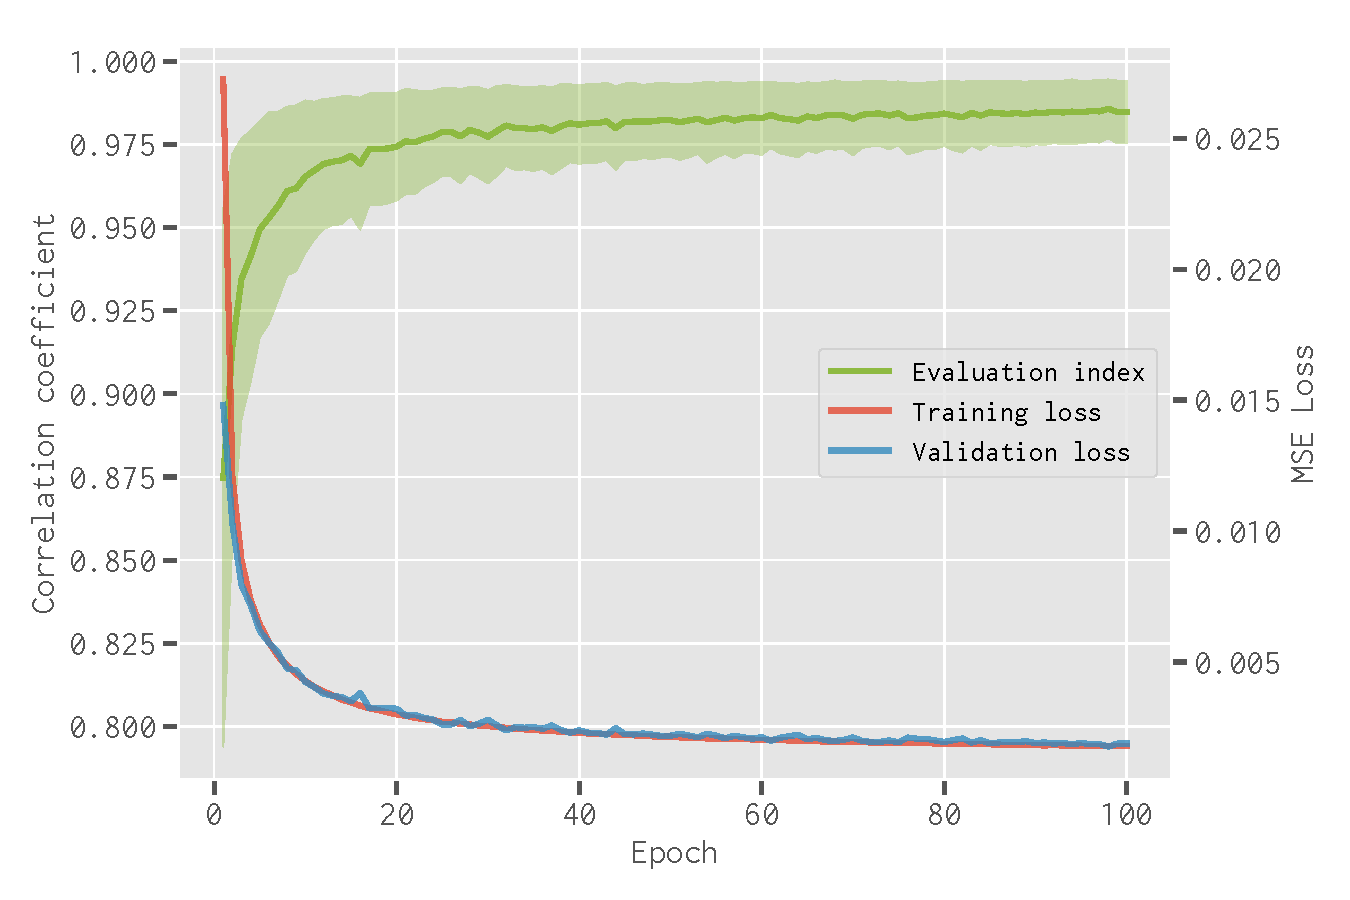
\includegraphics[width=\columnwidth]{cdae-train}
  \caption{\label{fig:train}%
    The correlation coefficient calculated on the validation set (the
    green line with the shaded region showing the standard deviation),
    training loss (the red line), and validation loss (the blue line)
    during the training of the CDAE.
  }
\end{figure}

The losses and the correlation coefficient calculated on the validation
set during the CDAE training are shown in \autoref{fig:train}.
The steadily decreasing losses and increasing correlation coefficient
suggest that the CDAE is well trained.
After training for 100 epochs, the CDAE achieves excellent performance
with a correlation coefficient of $\rho_{\R{cdae}} = \num{0.985 +- 0.009}$
on the validation set.
An example of the EoR signal separated by the trained CDAE is presented
in \autoref{fig:result}.
This separation example has a correlation coefficient of $\rho = 0.985$
and well demonstrates that the faint EoR signal can be separated with
high accuracy by our method.
Consequently, our deep-learning-based method by using the CDAE is able
to accurately separate the faint EoR signal in the presence of severe
foreground contamination and complicated instrumental effects.

\begin{figure}
  \centering
  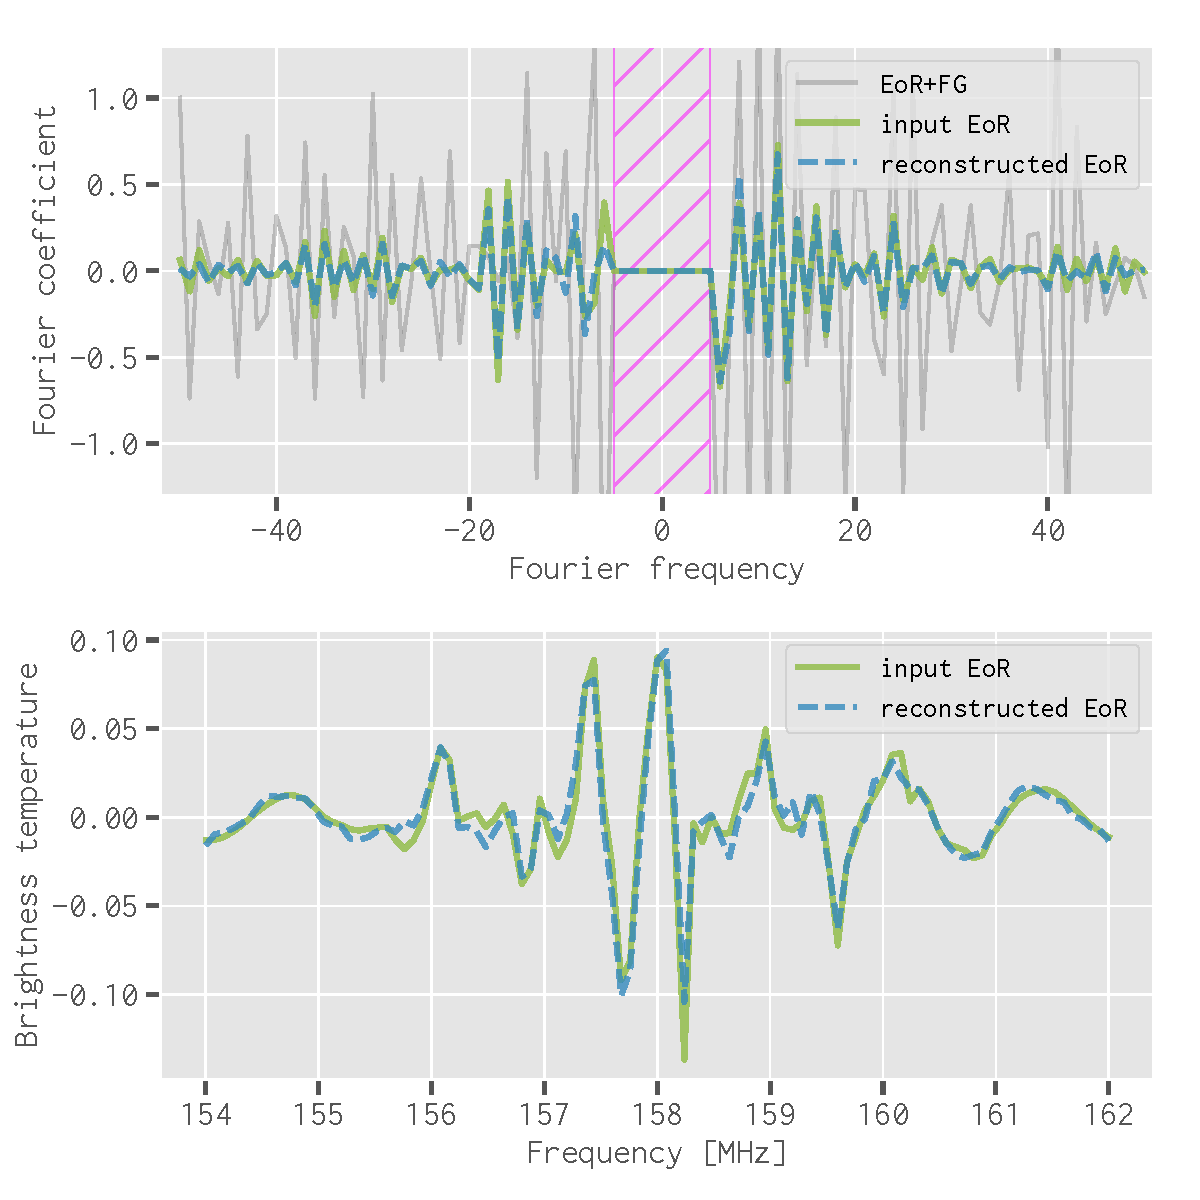
\includegraphics[width=\columnwidth]{eor-result}
  \caption{\label{fig:result}%
    An example of the EoR signal separated by the trained CDAE.
    \textbf{(top)} The labelled EoR signal (i.e., the ground truth;
    the blue line) and the separated EoR signal (the green line) in the
    Fourier domain where the CDAE training is performed.
    The grey line represents the input data to the CDAE that contains
    both the EoR signal and the foreground contamination.
    The magenta hatched region marks the lowest Fourier components that
    are excised in data preprocessing.
    \textbf{(bottom)} The labelled EoR signal (the blue line) and the
    separated EoR signal (the green line) transformed back to the
    observing frequency domain.
    The signals are very different to those shown in
    \autoref{fig:simudata}(a) because the Blackman-Nuttall window is
    applied along the frequency axis.
  }
\end{figure}


%%----------------------------------------------------------------------
\subsection{Comparison}
\label{sec:comparison}

In order to better demonstrate the excellent performance of our proposed
method, we carry out a comparison between our method and the traditional
polynomial fitting method.
Using the same data set simulated in \autoref{sec:data}, for each pixel
in the image cube of the addition of the EoR signal and the foreground
emission, a low-order polynomial is fitted along the frequency
dimension, the fitted value of which is then subtracted to uncover the
EoR signal.
We have tested polynomials of order from 2 (quadratic) to 5 (quintic),
and find that the quartic polynomial (order of 4) can give the
relatively best result.
However, the correlation coefficient calculated for the separated EoR
signal in such case is only $\rho_{\R{pfit}} = \num{0.241 +- 0.103}$,
which is rather small and indicates that the polynomial fitting method
performs very poor in separating the EoR signal.
As illustrated in \autoref{fig:simudata}, the complicated instrumental
effects seriously damage the spectral smoothness of the foreground
emission, causing rapid fluctuations of similar strength as or even
stronger than the EoR signal, therefore, it is unsurprising that the
polynomial fitting method gives very poor results.
On the contrary, our deep-learning-based method is superior and
by far outperforms the traditional polynomial fitting method.


%%======================================================================
\section{Conclusions}
\label{sec:conclusions}

We have demonstrated to use the CDAE to separate the faint EoR signal
that is buried in the overwhelming foreground contamination with the
complicated instrumental effects taken into account.
The proposed CDAE, which consists of a 7-layer encoder, a 7-layer
decoder, and one output layer, is trained on the simulated SKA images
and achieves excellent performance that is by far better than the
traditional polynomial fitting method.
In conclusion, our deep-learning-based method is able to accurately
separate the faint EoR signal in the presence of severe foreground
contamination and complicated instrumental effects.
In addition, the proposed CDAE is simple but powerful, exhibiting the
great potential of deep-learning-based methods to play an important
role in forthcoming EoR experiments.


%%======================================================================
\section*{Acknowledgements}

This work is supported by
the Ministry of Science and Technology of China
(grant Nos. 2018YFA0404601, 2017YFF0210903),
and the National Natural Science Foundation of China
(grant Nos. 11433002, 11621303, 11835009, 61371147).


%%======================================================================
%% References

\bibliographystyle{mnras}
\bibliography{references}


%%======================================================================
%% Appendix

% \appendix


%%======================================================================
% Don't change these lines
\bsp	% typesetting comment
\label{lastpage}
\end{document}

%% EOF
